\section{Reduce MPI Synchronisation}


\chapterDescription
  {
    Around 60 minutes.
  }
  {
    A working MPI code.
  }


Peano has very strong constraints on the master-worker and worker-master
communication as the data exchange between these two is synchronous. It imposes
a partial order. If that slows down your application (you see this from the
mpianalysis reports), you can kind of weaken the communication constraints. 
Often, some data is not required immediately, not required globally all the
time, or doesn't have to be 100\% correct at all algorithmic stages. This
chapter discusses some things that you can do then.
So we assume that you have proper load balancing.


\begin{smell}
We face a very strong synchronisation.
This materialises in very regular execution patterns
where each rank waits for rank 0 to start up a new traversal.
It can also be reported by Peano's performance analysis.
\end{smell}

\begin{center}
  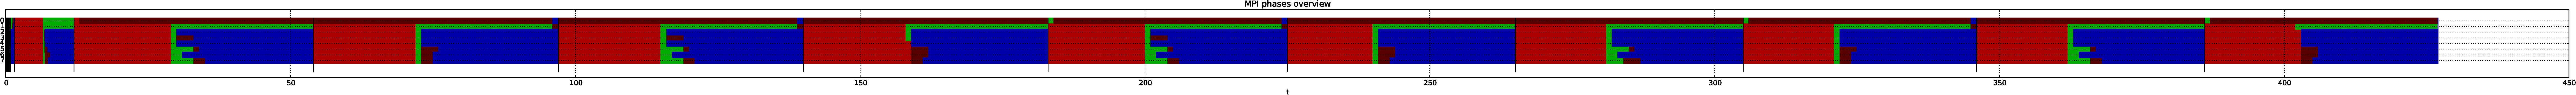
\includegraphics[width=0.9\textwidth]{63_mpi-synchronisation/mpi-phases-before.pdf}
\end{center}

\noindent
It also becomes obvious if you study how often a master has to work for its 
workers. 
In the picture below, only rank 0 synchronises the other ranks.
In this case, you have to weaken the global synchronisation.
If multiple of these edges pop up, it is time to weaken all the worker-master
synchronisations---unless you can identify that you have a load balancing issue.


\begin{center}
  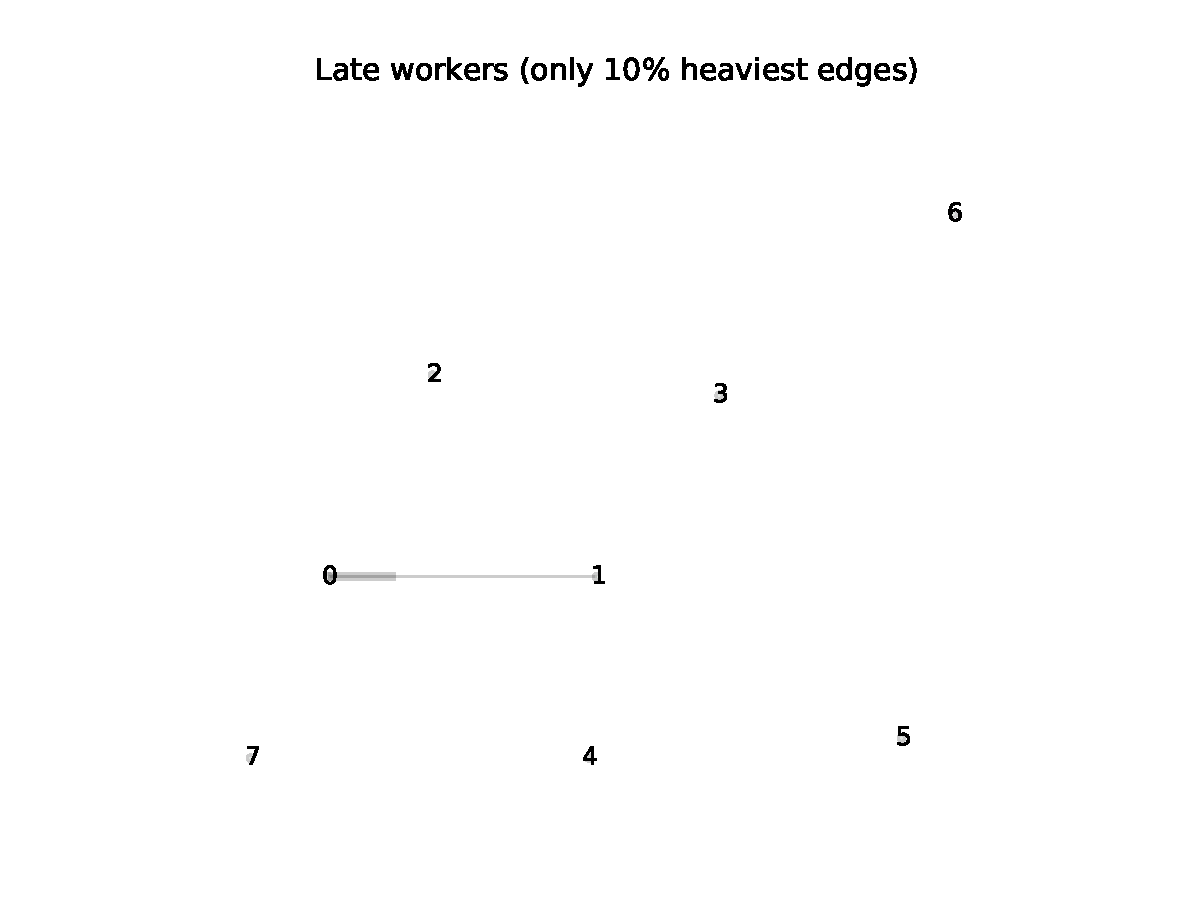
\includegraphics[width=0.5\textwidth]{63_mpi-synchronisation/master-worker-before.pdf}
\end{center}



\subsection{Postpone and tailor master-worker and worker-master data exchange}

In this section, we study the communication specification of the mappings. 
By default, they are set to the most general case:
Peano send away data from a local node if and only if it has traversed the whole local tree. 
In return, it requires all input data before it starts to traverse anything.

If you manage to send out data earlier, a rank's master can continue its local
traversal earlier.
If you manage to receive important data from the master, i.e.~from coarser
mesh levels, later, your rank can start its traversal right away when it is
informed which adapter is ran next.
This allows you to overlap computations more aggressively. 


\paragraph{Multiscale vertices and cells}

If a cell in the spacetree is deployed to another rank (grey cell in the sketch
below), the master continues to hold a replica of the deployed cell.
At the begin of a traversal, it sends the replica together with its parent cell
to the worker (blue instance) that is responsible for the actual data.
When the worker has finished its traversal, it sends the blue cell plus its
parent back to the master.
The same holds for the vertices adjacent to the cells.

\begin{center}
  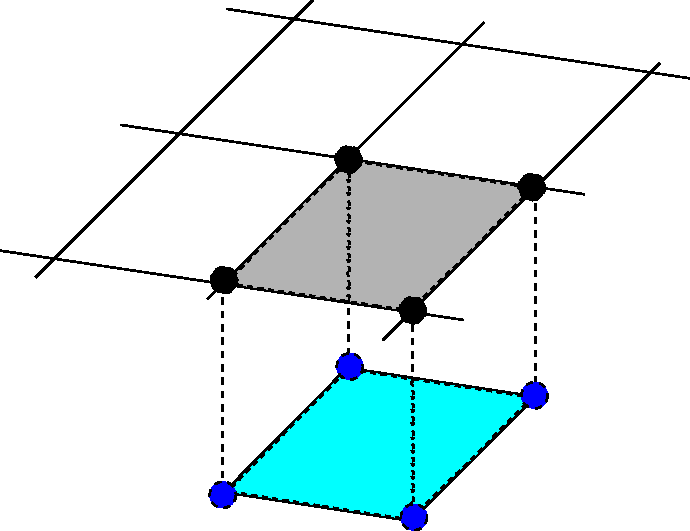
\includegraphics[width=0.35\textwidth]{63_mpi-synchronisation/master-worker.pdf}
\end{center}

\noindent
Such a workflow allows you to realise multiscale algorithms where information is
transferred through the cells or vertices from the master ot the worker and
back.
In return, the data exchange is rather critical as it runs synchronous.
The master is not allowed to fire up the worker to do its traversal before it
hasn't loaded all the vertices.
A similar reasoning holds the other way round.
Please note that the solver's state is exchanged along the very same lines,
i.e.~when we start up a worker and when the worker traversal terminates.


We notion that many codes do not require such a tight multiscale vertex
synchronisation.
If no multiscale data is exchanged at all, we do not need any of these
synchronous data sends and receives.
If we transfer data only through cells, we do not need the vertex copies before
we start the fine grid traversal.
We can wait until we do the very first \texttt{enterCell} on the worker.
Only if we need the copies of the vertices before the first
\texttt{touchVertexFirstTime}, we have to synchronise tightly.


\begin{remark}
In Peano, a cell that is deployed to a worker has exclusively refined adjacent
vertices. 
You can assume that a deployed cell (the greyish in the sketch) thus always is
refined.
\end{remark}


If you want tailor the data exchange, you have to open all the mappings you use
in your adapter.
There are two enumeration values that allow you specify exactly which data you
need at which time throughout a worker traversal.


\begin{remark}
Some codes may not skip multiscale data transfer all the time. See discussion in
the sections below on details.
\end{remark}


\subsection{Weaken synchronisation with global master}

\begin{center}
  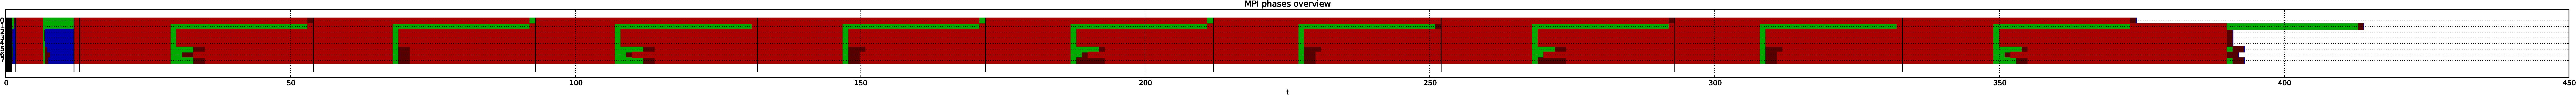
\includegraphics[width=0.9\textwidth]{63_mpi-synchronisation/mpi-phases-after.pdf}
\end{center}


\begin{smell}
The performance analysis reports on strong synchronisation and the traces show
that each new iteration on each rank coincides exactly with the start of a
global new step (vertical bars in plot).
\end{smell}


The global master (rank 0) is kind of a pulse generator for the whole code. 
Whenever the \texttt{runAsMaster} operation triggers \texttt{iterate}, it tells
each rank that handles a partition which adapter to use and to start its
traversal or wait for its master to trigger the traversal, respectively.
This is a very strong synchronisation.
Notably, no rank can continue to work with the next iteration unless rank 0 runs
into the next \texttt{iterate} as well.
There are basically two ways to improve this situation:

\begin{enumerate}
  \item Perform more than one time step with the same adapter and settings in a
  row. For this, use the integer argument of \texttt{iterate()}. Note that
  running multiple time steps switches off load balancing for this phase of the program.
  Obviously, this version works if and only if you run the same adapter several 
  times.
  \item You may alternatively find out that you don't need the rank 0 (that
  doesn't hold any data anyway) to wait for all the other ranks in each
  iteration. Often, you run for example a sequence of adapters and you require
  global data (such as global residual) only after the last run. 
  This second option (which is typically not a quick 'n dirty one) is discussed
  in the next subsection. 
\end{enumerate}



\subsection{Skip worker-master data transfer locally/sporadically}

We next discuss the decond variant.
Before we do so, we summarise typical smells that pop up once you have made 
your code run a fixed number of iterations:

\begin{smell}
You run multiple iterations with one \texttt{iterate} command but nevertheless
 \begin{itemize}
  \item the performance analysis identifies strong synchronisation or
  \item shows that some ranks permanently are late with their boundary data
  while the MPI trace shows that the traversals are kind of in sync.
 \end{itemize}
\end{smell}

\begin{center}
  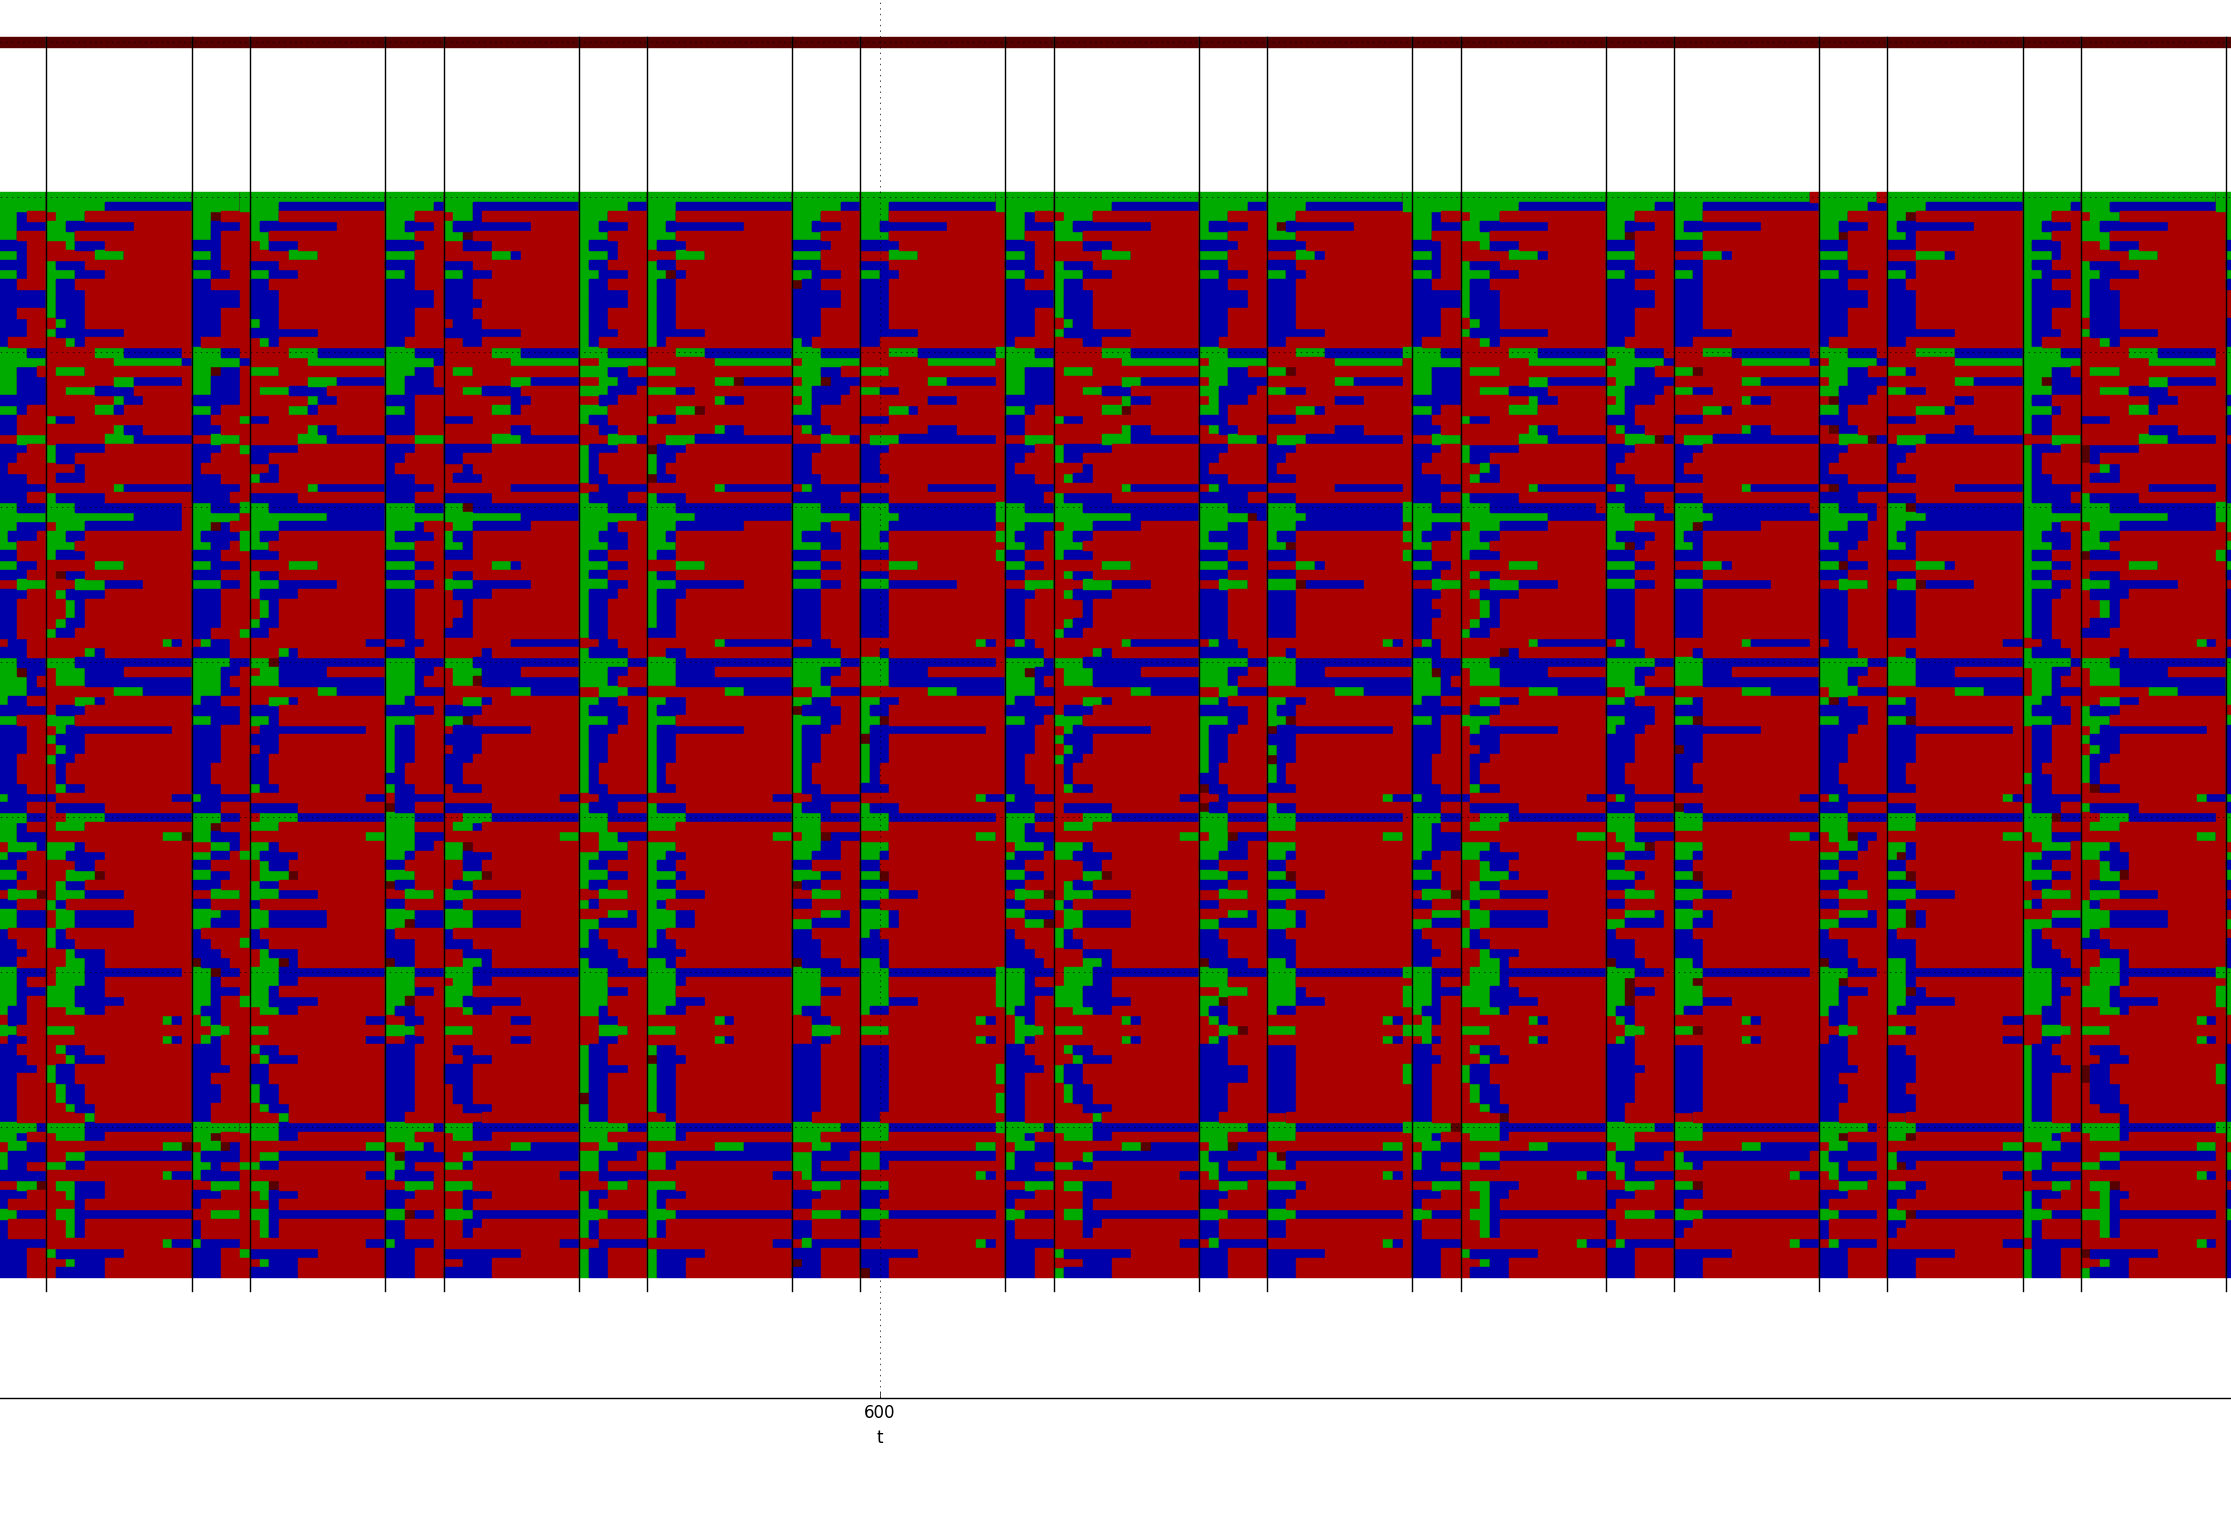
\includegraphics[width=0.7\textwidth]{63_mpi-synchronisation/no-skip-of-reduction.png}
\end{center}

\noindent
We see in the example above that the execution phases are in sync while the
report finds no later worker-master relation. 
Furthermore, we see an oscillating pattern: every second iteration lasts
significantly longer which materialises in zig zag timings for individual steps,
too.

Our goal in this step is to break up this synchronisation further which,
depending on your smell
\begin{itemize}
  \item eliminates late workers or
  \item allows more ranks to aggressively finish their boundary data exchange
  and thus free the interconnects from traffic.
\end{itemize}



If you want to realise the second variant, you have to
ensure that all mappings you use (also the predefined ones) return false in
\texttt{prepareSendToWorker(...)}.
  
\begin{remark}
  If you want to validate that reductions have been skipped, switch on the log
  info of 
  \texttt{peano::grid::nodes::Node::updateCellsParallel}
  \texttt{StateBeforeStoreForRootOfDeployedSubtree}.
\end{remark}


\noindent
Please be aware that reduction are skipped by the kernel if and only if all
mappings allow the kernel to switch off the reduction.
Furthermore, load balancing has to be disabled.
If you want to load balance, master and worker ranks have to communicate with
each other and may not skip any data/status exchange.

We also observe that the reduction skips often only change the communication
profile but do not speed up the computation. 
Often it is only a preparatory step to switch off boundary data exchange
afterwards.
Once this is done, you should get a profile as below. 
It is more or less completely asynchronous, and all data exchange (blue) is
hidden in the background, i.e.~not visible anymore:




Peano relies on a modified depth-first (dfs) traversal. The parallel variant also is a dfs, but whenever the dfs traversal encounters a remote node, it makes another mpi rank traverse the corresponding spacetree, while it continues itself with the local subtree. Before is ascends again, it checks whether the remote subtree traversals have terminates as well. As a result, it is important to split up the tree on an as coarse level as possible to obtain a high concurrency Level. Let's study a toy problem in 1d:


getCoarsestGridLevelOfAllSolvers()
